
\begin{center}

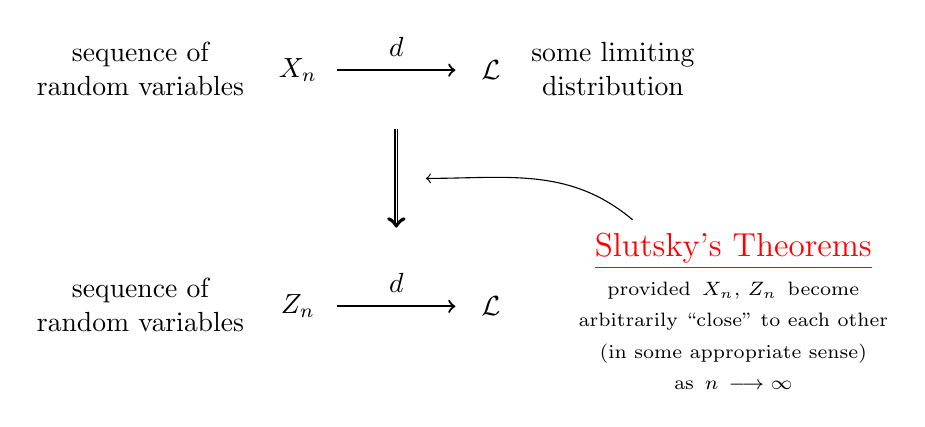
\begin{tikzpicture}

\pause
\node at (2,0) {$Z_{n}$};
\node at (0,0.2) {sequence of};
\node at (0,-0.2) {random variables};
\node at (2,3) {$X_{n}$};
\node at (0,3.2) {sequence of};
\node at (0,2.8) {random variables};

\pause
\node at (3.25,3.3) {$d$};
\draw [->,thick] (2.5,3) -- (4,3);
\node at (4.45,3.0) {$\mathcal{L}$};
\node at (6,3.2) {some limiting};
\node at (6,2.8) {distribution};

\pause
\node at (7.53,0.7) {\large\color{red}\underline{Slutsky's Theorems}};
\draw [->,double] (3.25,2.25) -- (3.25,1.0);
\draw [<-] (3.625,1.625) to [out=0,in=140] (6.25,1.1);
\node at (3.25,0.3) {$d$};
\draw [->,thick] (2.5,0) -- (4,0);
\node at (4.45,0) {$\mathcal{L}$};

\pause
\node at (7.53,0.2) {\scriptsize provided \,$X_{n},\,Z_{n}$\, become};
\node at (7.53,-0.2) {\scriptsize arbitrarily ``close'' to each other};
\node at (7.53,-0.6) {\scriptsize (in some appropriate sense)};
\node at (7.53,-1.0) {\scriptsize as \,$n\,\longrightarrow \infty$};

%%%%%%%%%%%%%
%\pause
%\node at (7.85,0.275) {\scriptsize H\'{a}jek's sampling design};

%\pause
%\node at (7.86,0.0) {\tiny (H\'{a}jek's fundamental inequality)};
%\pause
%\node at (7.53,-0.4) {\scriptsize\color{gcblue}$n\,,\;N-n\,\longrightarrow \infty$};

\onslide<1-> % added to force frame number to be displayed at footline.
\end{tikzpicture}

\end{center}
